\documentclass[12pt]{beamer}
\usepackage[utf8]{inputenc} % style d'écriture
\usepackage[T1]{fontenc}      % package
\usepackage[french]{babel}  % package pour langue française
\usepackage{graphicx}
\usepackage{subcaption}
\usepackage{url}
\usepackage{color}
\usepackage{geometry}
\usepackage{amssymb}
\usepackage{multirow, makecell}
\usepackage{listings}

% William PENSEC, étudiant en Master 2 LSE 2020/2021

\usetheme[secheader]{Madrid}
\beamertemplatenavigationsymbolsempty
\setbeamertemplate{frametitle continuation}{}

\lstset{
  aboveskip=5mm,
  belowskip=-2mm,
  basicstyle=\footnotesize,
  breakatwhitespace=false,
  breaklines=true,
  captionpos=b,
  commentstyle=\color{red},
  deletekeywords={...},
  escapeinside={\%*}{*)},
  extendedchars=true,
  framexleftmargin=16pt,
  framextopmargin=3pt,
  framexbottommargin=6pt,
  frame=tb,
  keepspaces=true,
  keywordstyle=\color{blue},
  language=C++,
  literate=
  {²}{{\textsuperscript{2}}}1
  {⁴}{{\textsuperscript{4}}}1
  {⁶}{{\textsuperscript{6}}}1
  {⁸}{{\textsuperscript{8}}}1
  {€}{{\euro{}}}1
  {é}{{\'e}}1
  {è}{{\`{e}}}1
  {ê}{{\^{e}}}1
  {ë}{{\"{e}}}1
  {É}{{\'{E}}}1
  {Ê}{{\^{E}}}1
  {û}{{\^{u}}}1
  {ù}{{\`{u}}}1
  {â}{{\^{a}}}1
  {à}{{\`{a}}}1
  {á}{{\'{a}}}1
  {ã}{{\~{a}}}1
  {Á}{{\'{A}}}1
  {Â}{{\^{A}}}1
  {Ã}{{\~{A}}}1
  {ç}{{\c{c}}}1
  {Ç}{{\c{C}}}1
  {õ}{{\~{o}}}1
  {ó}{{\'{o}}}1
  {ô}{{\^{o}}}1
  {Õ}{{\~{O}}}1
  {Ó}{{\'{O}}}1
  {Ô}{{\^{O}}}1
  {î}{{\^{i}}}1
  {Î}{{\^{I}}}1
  {í}{{\'{i}}}1
  {Í}{{\~{Í}}}1,
  morekeywords={*,...},
  numbers=left,
  numbersep=10pt,
  numberstyle=\tiny\color{black},
  rulecolor=\color{black},
  showspaces=false,
  showstringspaces=false,
  showtabs=false,
  stepnumber=1,
  stringstyle=\color{gray},
  tabsize=4,
  title=\lstname,
}

\title[Compte rendu de stage n\textsuperscript{o}14]{Coopération de drones dans un système hétérogène}
\subtitle{Compte rendu de stage n\textsuperscript{o}14}
\author{William \textsc{Pensec}}
%\author{William \textsc{Pensec}}
%\author{William \textsc{Pensec}}
\institute[Lab-STICC]{Lab-Sticc}
\date{\today}

%\AtBeginSection[]
%{
%\begin{frame}<beamer>{Sommaire}
%\tableofcontents[currentsection,currentsubsection, 
%    hideothersubsections, 
%    sectionstyle=show/shaded,
%]
%\end{frame}
%}

\begin{document}
	% ---------------------------------------------------------------- %
	\begin{frame}
		\begin{titlepage}
			\begin{figure}[H]
				\centering
				
\includegraphics[scale=.15]{labsticc.png}
				\hspace{3cm}
				
\includegraphics[scale=.3]{ubo.png}
			\end{figure}
		\end{titlepage}
	\end{frame}
	
	% ---------------------------------------------------------------- %
	\section*{Sommaire}
	\begin{frame}
		\frametitle{Sommaire}
		\begin{center}
			\tableofcontents
		\end{center}
	\end{frame}
	%
	% ---------------------------------------------------------------- %
	\section{Mouvements d'un point A à un point B}
	\begin{frame}[allowframebreaks]
	    % Finir mouvements du drone d'un point A vers point B
	    % Préparation article
	    % Préparation rapport de stage
	    % Tester scenario/scenarii mouvement de drone
	    % Faire un dataset des anomalies (entre 4 et 10)
	    %   - pas de tube sur la plate-forme
	    %   - pas de bouchon sur la plate-forme
	    %   - levier qui reste bloqué à un endroit
	    % Utiliser LeNET-5 pour réseau de neurones
	    % Magnetometre : X (Est / Ouest) , Y (Nord / Sud), Z (Profondeur)
	    
	     \begin{block}{Utilisation du magnétomètre}
	        \begin{itemize}
	            \setbeamertemplate{itemize item}[triangle]
	            \item Valeur trouvée qui correspond à la boussole
	            \item Documentation très incomplète
	            \item Valeur comprise entre 0 et 0.9999 si on va du Nord au Sud par l'Est (0.69)
	            \item Valeur comprise entre 0 et -0.9999 si on va du Nord au Sud par l'Ouest (-0.86)
	        \end{itemize}
	    \end{block}
	\end{frame}
	%
	% ---------------------------------------------------------------- %
	\begin{frame}[allowframebreaks]
	    \begin{figure}
		    \centering
		    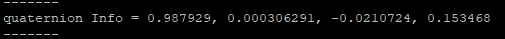
\includegraphics[width=1\linewidth]{quat.png}
	    \end{figure}
	    
	    \begin{figure}
		    \centering
		    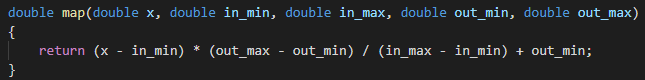
\includegraphics[width=1\linewidth]{map.png}
	    \end{figure}
	    
	    \begin{figure}
		    \centering
		    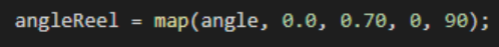
\includegraphics[width=1\linewidth]{mapused.png}
	    \end{figure}
	    
	    \begin{figure}
		    \centering
		    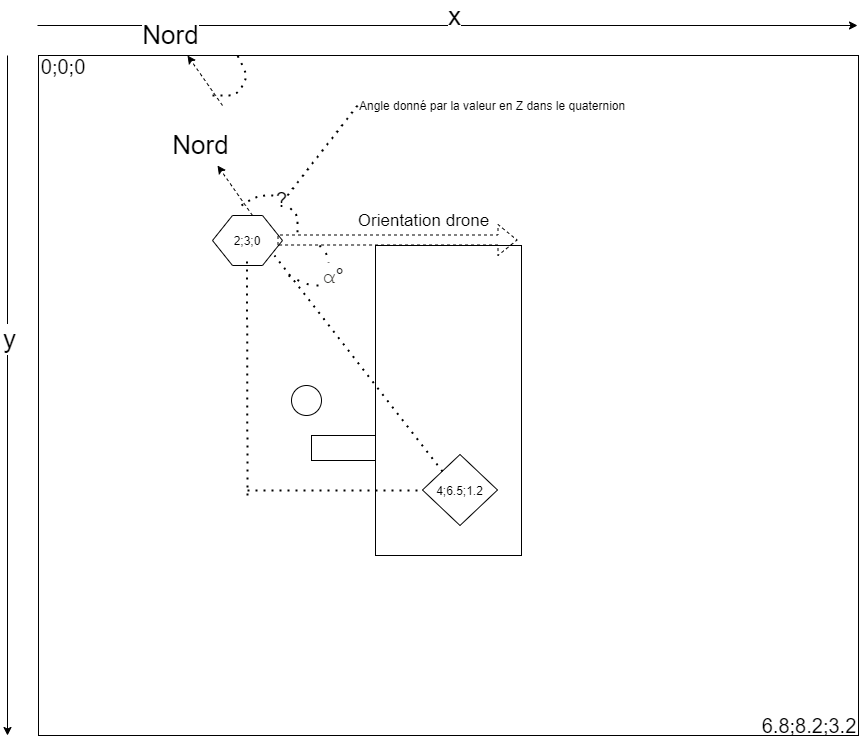
\includegraphics[width=0.8\linewidth]{schema.png}
	    \end{figure}
	    
	    \begin{figure}
		    \centering
		    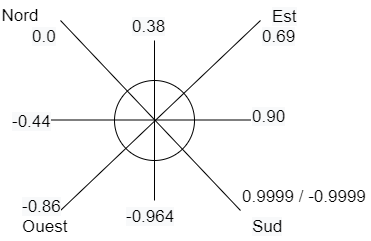
\includegraphics[width=0.5\linewidth]{schema1.jpg}
	    \end{figure}
	\end{frame}
	%
	% ---------------------------------------------------------------- %
\end{document}